\documentclass[tikz,border=1.25mm]{standalone}
\usetikzlibrary{matrix, positioning, shapes, fit, shapes.geometric, backgrounds, arrows.meta}
\usepackage{amssymb}

\definecolor{kellygreen}{rgb}{0.3, 0.73, 0.09}
\definecolor{gray}{rgb}{0.54, 0.54, 0.54}
\definecolor{slate}{rgb}{0.094,0.094,0.112}
\definecolor{cobalt}{rgb}{0.244,0.364,0.972}

\begin{document}

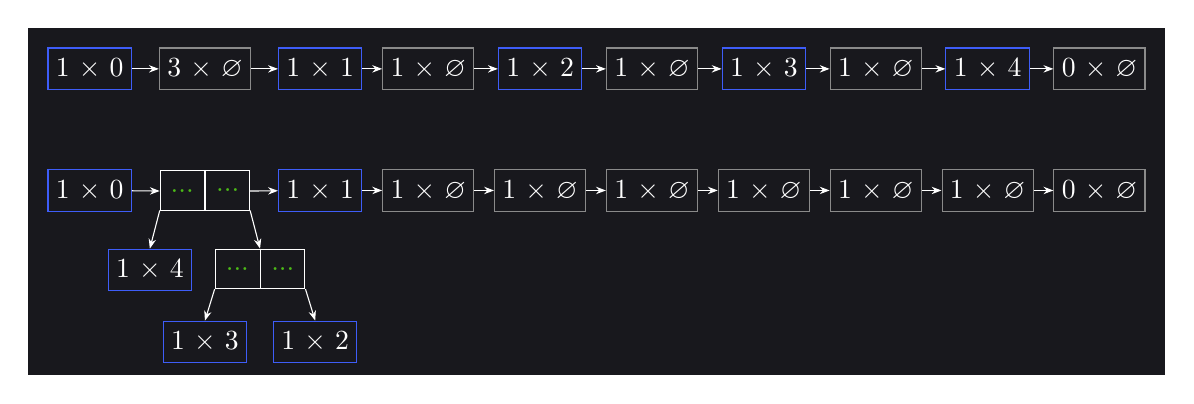
\begin{tikzpicture}[
  background rectangle/.style={fill=slate},
  show background rectangle,
  every node/.style={
    color=cobalt,
    text=white,
    draw,
    inner sep=1mm,
    minimum height=5.3mm,
    minimum width=5mm,
    text height=2mm,
    text depth=0mm
  },
  move arrow/.style={
    -{Stealth[length=1.25mm]},
    draw=white
  }
]

\matrix[
	matrix of nodes,
	nodes in empty cells,
	column sep=2.5mm,
	row sep=10mm,
	draw=none
] (m) {
    1 $\times$ 0 & |[color=gray,text=white]| 3 $\times$ $\varnothing$ & 1 $\times$ 1 & |[color=gray,text=white]| 1 $\times$ $\varnothing$ & 1 $\times$ 2 & |[color=gray,text=white]| 1 $\times$ $\varnothing$ & 1 $\times$ 3 & |[color=gray,text=white]| 1 $\times$ $\varnothing$ & 1 $\times$ 4 & |[color=gray,text=white]| 0 $\times$ $\varnothing$ \\
    1 $\times$ 0 &
    \node(spl)[alias=spl0,below=-2mm,draw=none,minimum height=5mm,minimum width=10mm,align=center, every nodepart/.style={inner xsep=2mm}]
    {\tikz{\node[rectangle split,rectangle split horizontal,rectangle split parts=2,draw,inner sep=0mm,minimum height=5mm,minimum width=5mm,align=center,text depth=1.6mm,color=white,text=kellygreen,inner xsep=1.35mm]
    {\nodepart{one} ... \nodepart{two} ...};}};
    & 1 $\times$ 1 & |[color=gray,text=white]| 1 $\times$ $\varnothing$ & |[color=gray,text=white]| 1 $\times$ $\varnothing$ & |[color=gray,text=white]| 1 $\times$ $\varnothing$ & |[color=gray,text=white]| 1 $\times$ $\varnothing$ & |[color=gray,text=white]| 1 $\times$ $\varnothing$ & |[color=gray,text=white]| 1 $\times$ $\varnothing$ & |[color=gray,text=white]| 0 $\times$ $\varnothing$ \\
};

\node(n1x4)[draw, below=3.25mm of spl0, xshift=-7mm] {1 $\times$ 4};

\node(spl)[alias=spl1,below=3.25mm of spl0,xshift=7mm,rectangle split,rectangle split horizontal,rectangle split parts=2,draw,inner sep=0mm,minimum height=5mm,minimum width=5mm,align=center,text depth=1.6mm,color=white,text=kellygreen,inner xsep=1.35mm] {\nodepart{one} ... \nodepart{two} ...};

\node(n1x3)[draw, below=4mm of spl1, xshift=-7mm] {1 $\times$ 3};
\node(n1x2)[draw, below=4mm of spl1, xshift=7mm] {1 $\times$ 2};

\draw[move arrow] ([yshift=1.6mm, xshift=1.1mm]spl0.south west) -- (n1x4.north);
\draw[move arrow] ([yshift=1.6mm, xshift=-1.1mm]spl0.south east) -- (spl1.north);
\draw[move arrow] (spl1.south west) -- (n1x3.north);
\draw[move arrow] (spl1.south east) -- (n1x2.north);

\draw[move arrow] (m-1-1) -> (m-1-2);
\draw[move arrow] (m-1-2) -> (m-1-3);
\draw[move arrow] (m-1-3) -> (m-1-4);
\draw[move arrow] (m-1-4) -> (m-1-5);
\draw[move arrow] (m-1-5) -> (m-1-6);
\draw[move arrow] (m-1-6) -> (m-1-7);
\draw[move arrow] (m-1-7) -> (m-1-8);
\draw[move arrow] (m-1-8) -> (m-1-9);
\draw[move arrow] (m-1-9) -> (m-1-10);

\draw[move arrow] (m-2-1) -> ([yshift=1.5mm, xshift=1.1mm]spl0.west);
\draw[move arrow] ([yshift=1.5mm, xshift=-1.1mm]spl0.east) -> (m-2-3);
\draw[move arrow] (m-2-3) -> (m-2-4);
\draw[move arrow] (m-2-4) -> (m-2-5);
\draw[move arrow] (m-2-5) -> (m-2-6);
\draw[move arrow] (m-2-6) -> (m-2-7);
\draw[move arrow] (m-2-7) -> (m-2-8);
\draw[move arrow] (m-2-8) -> (m-2-9);
\draw[move arrow] (m-2-9) -> (m-2-10);

\end{tikzpicture}

\end{document}
